\documentclass[tikz,border=8pt]{standalone}
\usepackage{amsmath,amssymb}
\usetikzlibrary{arrows.meta,automata,positioning,quotes}
\begin{document}
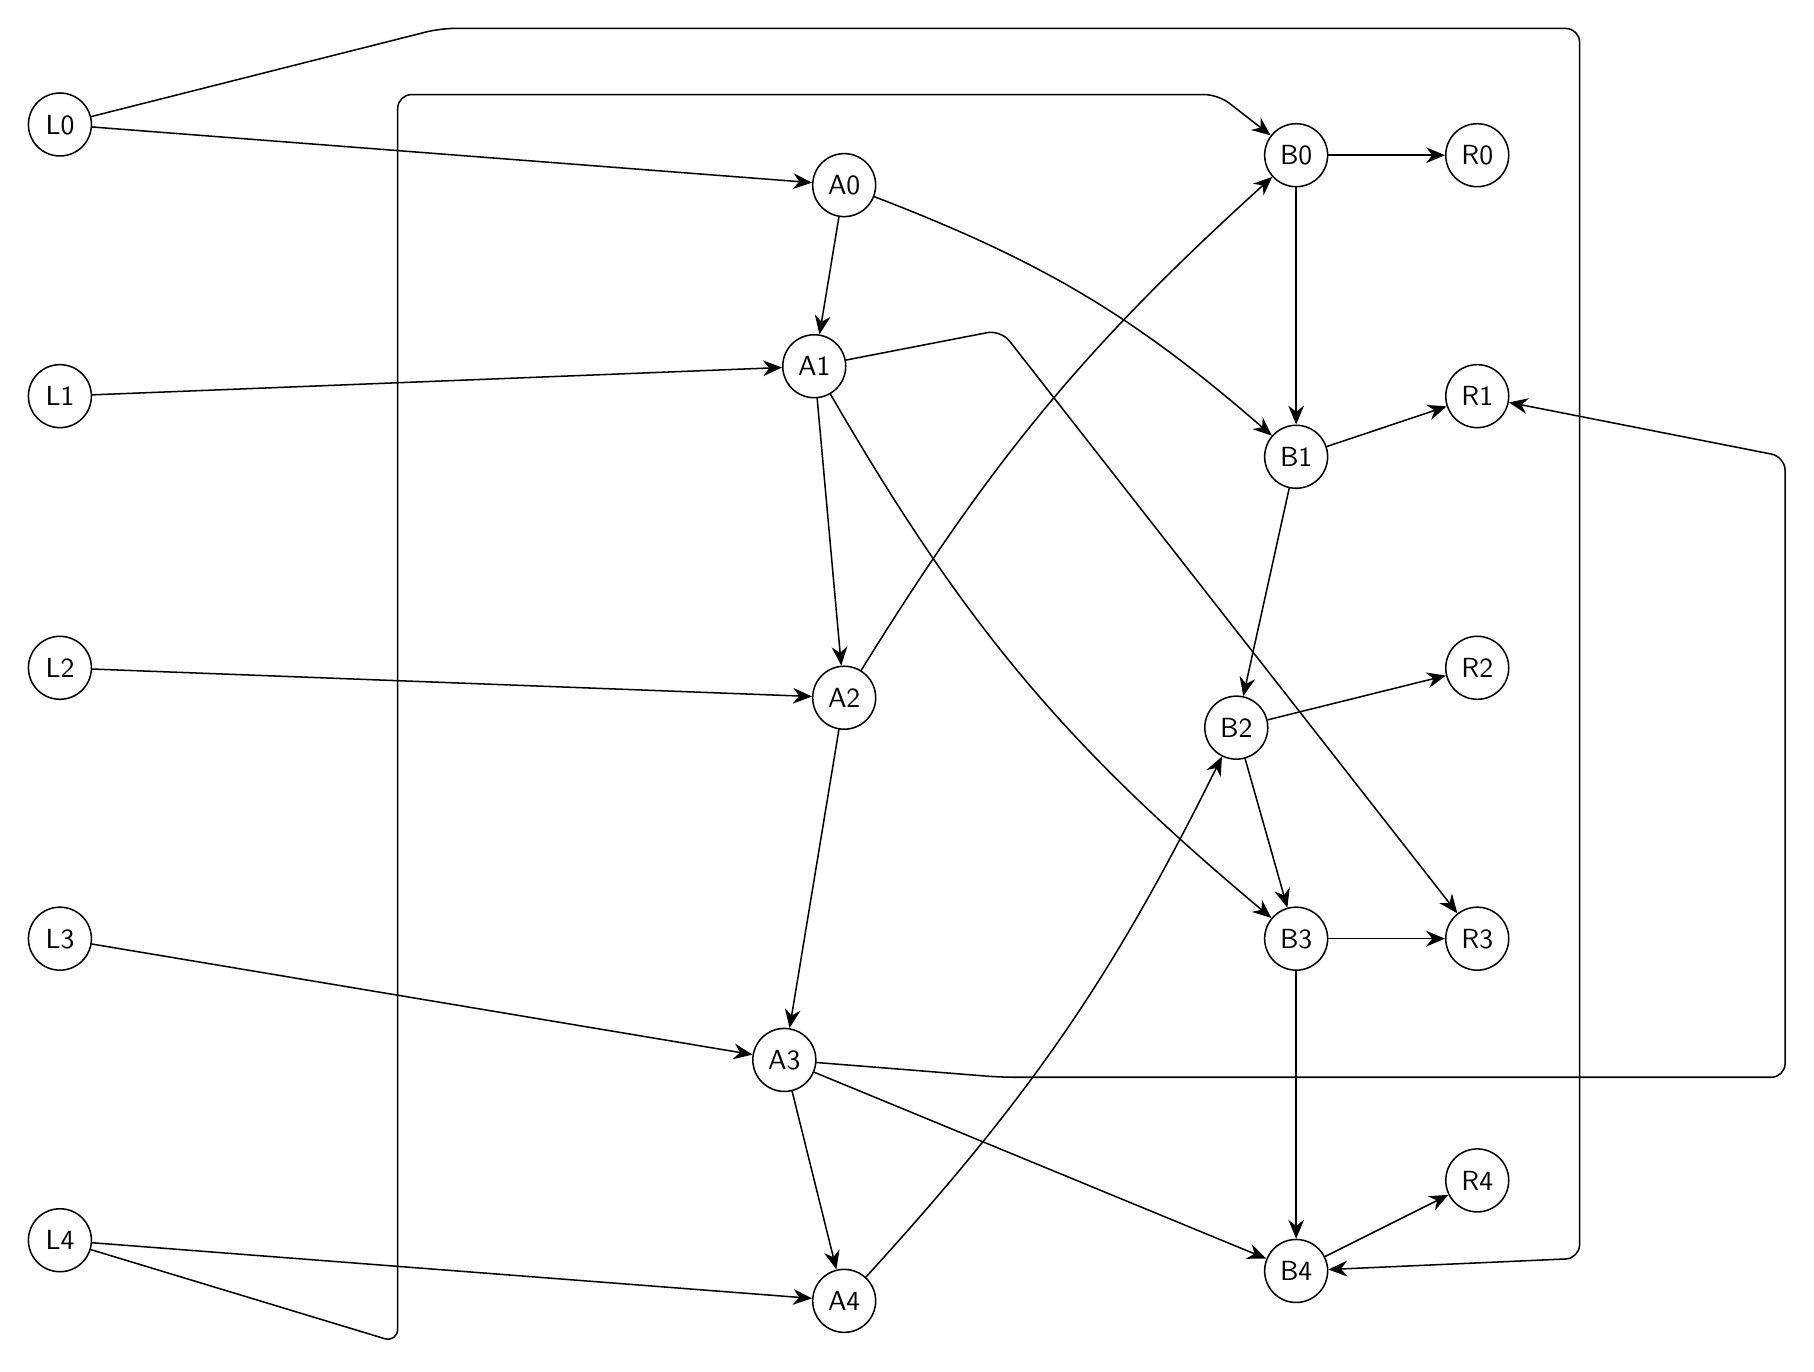
\begin{tikzpicture}[x=1cm,y=1cm]
\tikzset{
  graphnode/.style={circle,draw=black,line width=0.55pt,minimum size=8mm,inner sep=1pt,font=\sffamily},
  graphedge/.style={draw=black,line width=0.55pt,line cap=round,line join=round},
  directed/.style={graphedge,-{Stealth[length=2.4mm,width=2.0mm]}},
  undirected/.style={graphedge}
}
\node[graphnode] (n_L0) at (-12.01,7.26) {L0};
\node[graphnode] (n_L1) at (-12.01,3.81) {L1};
\node[graphnode] (n_L2) at (-12.01,0.36) {L2};
\node[graphnode] (n_L3) at (-12.01,-3.08) {L3};
\node[graphnode] (n_L4) at (-12.01,-6.91) {L4};
\node[graphnode] (n_R0) at (5.99,6.87) {R0};
\node[graphnode] (n_R1) at (5.99,3.81) {R1};
\node[graphnode] (n_R2) at (5.99,0.36) {R2};
\node[graphnode] (n_R3) at (5.99,-3.08) {R3};
\node[graphnode] (n_R4) at (5.99,-6.15) {R4};
\node[graphnode] (n_A0) at (-2.05,6.49) {A0};
\node[graphnode] (n_A1) at (-2.43,4.19) {A1};
\node[graphnode] (n_A2) at (-2.05,-0.02) {A2};
\node[graphnode] (n_A3) at (-2.81,-4.62) {A3};
\node[graphnode] (n_A4) at (-2.05,-7.68) {A4};
\node[graphnode] (n_B0) at (3.69,6.87) {B0};
\node[graphnode] (n_B1) at (3.69,3.04) {B1};
\node[graphnode] (n_B2) at (2.93,-0.40) {B2};
\node[graphnode] (n_B3) at (3.69,-3.08) {B3};
\node[graphnode] (n_B4) at (3.69,-7.30) {B4};
\draw[directed] (n_L0) -- (n_A0);
\draw[directed] (n_L1) -- (n_A1);
\draw[directed] (n_L2) -- (n_A2);
\draw[directed] (n_L3) -- (n_A3);
\draw[directed] (n_L4) -- (n_A4);
\draw[directed] (n_B0) -- (n_R0);
\draw[directed] (n_B1) -- (n_R1);
\draw[directed] (n_B2) -- (n_R2);
\draw[directed] (n_B3) -- (n_R3);
\draw[directed] (n_B4) -- (n_R4);
\draw[directed] (n_A0) to[bend left=10] (n_B1);
\draw[directed] (n_A1) to[bend right=10] (n_B3);
\draw[directed] (n_A2) to[bend left=8] (n_B0);
\draw[directed] (n_A3) -- (n_B4);
\draw[directed] (n_A4) to[bend right=8] (n_B2);
\draw[directed] (n_A0) -- (n_A1);
\draw[directed] (n_A1) -- (n_A2);
\draw[directed] (n_A2) -- (n_A3);
\draw[directed] (n_A3) -- (n_A4);
\draw[directed] (n_B0) -- (n_B1);
\draw[directed] (n_B1) -- (n_B2);
\draw[directed] (n_B2) -- (n_B3);
\draw[directed] (n_B3) -- (n_B4);
\draw[directed,rounded corners=5pt] (n_L0) -- (-7.18,8.48) -- (7.29,8.48) -- (7.29,-7.14) -- (n_B4);
\draw[directed,rounded corners=5pt] (n_L4) -- (-7.72,-8.21) -- (-7.72,7.64) -- (2.70,7.64) -- (n_B0);
\draw[directed,rounded corners=5pt] (n_A1) -- (-0.06,4.65) -- (n_R3);
\draw[directed,rounded corners=5pt] (n_A3) -- (-0.06,-4.84) -- (9.90,-4.84) -- (9.90,3.04) -- (n_R1);
\end{tikzpicture}
\end{document}
